
%% Copyright 2005 G. W. Knor
%%This work may be distributed and/or modified under the
% conditions of the LaTeX Project Public License, either version 1.3
% of this license or (at your option) any later version.
% The latest version of this license is in
% http://www.latex-project.org/lppl.txt
% and version 1.3 or later is part of all distributions of LaTeX
% version 2005/12/01 or later.
%%This work has the LPPL maintenance status "maintained".
%%The Current Maintainer of this work is G. W. Knor.

\documentclass{beamer}
\usepackage{graphicx}
\usepackage{amsmath} % provides \text{<stuff>} which prints <stuff> in text mode
\usepackage{sidecap}
\usepackage{courier}
\usepackage{listings}
\usepackage{hyperref}
\usepackage[utf8]
{inputenc}
\lstset{
    breaklines=true,
    breakatwhitespace=true,
    postbreak=\raisebox{0ex}[0ex][0ex]{
        \ensuremath{
            \color{red}\hookrightarrow\space
        }
    }
}
\setcounter{tocdepth}{1}

\definecolor{keywords}{RGB}{255,0,90}
\definecolor{comments}{RGB}{0,0,113}
\definecolor{red}{RGB}{160,0,0}
\definecolor{green}{RGB}{0,150,0}

\lstset{
    language=Python,
    basicstyle=\ttfamily\footnotesize,
    keywordstyle=\color{keywords},
    commentstyle=\color{comments},
    stringstyle=\color{red},
    showstringspaces=false,
    identifierstyle=\color{green}
}


\title{Containerize your world}
\author{Dariusz Śmigiel}
\date{PyCon PL 2015}
\usetheme{Warsaw}
\usecolortheme{beaver}

\begin{document}
\begin{frame}
\titlepage
\end{frame}

\section{History}
\subsection{Introduction}
\begin{frame}
\begin{itemize}
\item Full virtualization
\item Para-Virtualization
\item Operating system-level virtualization
\item Hardware-Assisted Virtualization
\end{itemize}
\end{frame}

\subsection{Origins}
\begin{frame}
1964 - IBM developed Virtual Machine Monitor \\
\pause
\begin{itemize}
\item partitions allowed mainframes to multitask
\item run multiple applications and processes at the same time
\end{itemize}
\pause
Why? \\
\begin{itemize}
\item Very expensive hardware
\item underutilization was a problem -- provide way to fully leverage investment
\end{itemize}
\end{frame}

\subsection{Cheap Hardware}
\begin{frame}
1980s - 1990s \\
\begin{itemize}
\item hardware is cheaper
\pause
\item x86 architecture doesn't support virtualization
\pause
\item relic of previous era
\pause
\item client-server applications
\pause
\item one application per server
\end{itemize}
\end{frame}

\subsection{Problems}
\begin{frame}
\begin{itemize}
\item Low Utilization ~5\%-15\%
\pause
\item Extra costs of power and cooling requirements
\pause
\item IT management costs
\pause
\item Insufficient failover and disaster protection
\end{itemize}
\end{frame}

\section{Terminology}
\subsection{Virtual Machine}
\begin{frame}
Host server \\
Underlying hardware, provides computing resources:
\begin{itemize}
\item processor
\item memory
\item disk
\item network
\item ...
\end{itemize}
Guest Virtual Machine \\
Separate and independent instance of an operating system and application software
\end{frame}

\subsection{Virtual Machine Monitor}
\begin{frame}
Virtual Machine Monitor (hypervisor) - virtualizing fill set of hardware resources, including:
\begin{itemize}
\item processor(s)
\item memory
\item storage
\item peripheral devices
\end{itemize}
\end{frame}

\subsection{Popek and Goldberg Criteria}
\begin{frame}
1974 - "Formal Requirements for Virtualizable Third Generation Architectures"
\\ \pause
Set of conditions sufficient for a computer architecture to support system virtualization efficiently. \\
\begin{itemize}
\item Equivalence/Fidelity - software should exhibit behavior essentially identical to equivalent hardware (barring timing effects);
\pause
\item Efficiency/Performance - vast majority of machine instructions must be executed by hardware, without VMM intervention
\pause
\item Resource Control/Safety - VMM must be in complete control of virtualized resources.
\end{itemize}
\end{frame}


\subsection{CPU Protection Levels}
\begin{frame}
x86 architecture offers protection levels (rings). \\
\pause
Ring 0 has the highest privilege -- operating system kernel (system space, kernel mode or supervisor mode) \\
\pause
Ring 1-3 run appications -- typically Ring 3.
\pause
\begin{center}
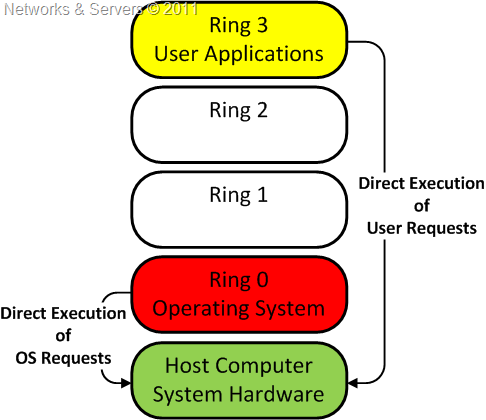
\includegraphics[width=0.5\textwidth]{images/ring0.png}
\end{center}
\end{frame}

\subsection{Virtualization problems}
\begin{frame}
OS expects to be running on bare-metal hardware (Ring 0). \\
Some instructions can't be virtualized: have different semantics when not executed in Ring 0. \\
Problem with trapping and translating instruction at runtime.
\end{frame}

\subsection{VMware FTW!}
\begin{frame}
In 1998, VMware virtualized x86 platform. \\
\pause
Developed binary translation techniques: allow running VMM in Ring 0 (isolation and performance). \\
\pause
Operating System is moved to user-level ring (with greater privilege than Ring 3, but less than Ring 0).
\pause
\begin{center}
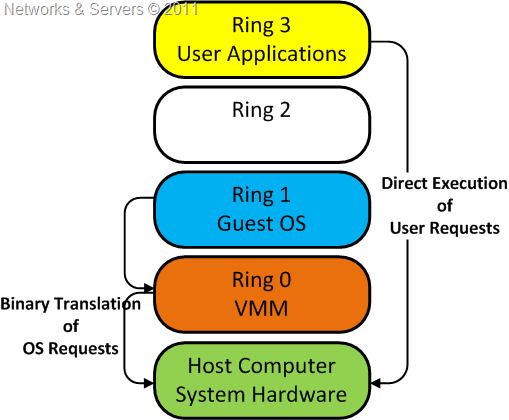
\includegraphics[width=0.5\textwidth]{images/ring3.png}
\end{center}
\end{frame}

\section{Full virtualization}
\subsection{Introduction}
\begin{frame}
Guest OS makes sytem calls to emulated hardware. \\
\pause
Calls are intercepted by virtualization hypervisor which maps them onto real, underlying hardware. \\
\pause
Hypervisor provides complete independence and autonomy. \\
\pause
Hypervisor monitors and controls physical resources.
\end{frame}

\subsection{Types of virtualization}
\begin{frame}
\begin{itemize}
\item Type 1 Hypervisor -- bare-metal virtualization
\item Type 2 Hypervisor -- guest OS virtualization
\item Embedded Hypervisor -- Kernel Linux Virtualization
\end{itemize}
\end{frame}

\subsection{Type 2 Hypervisor}
\begin{frame}
Guest OS virtualization (Hosted Virtualization). \\
\pause
OS provides abstraction layer, that allows other OSes to reside within - creating VMs. \\
\pause
Examples: Virtualbox, VMware Server, Microsoft Virtual PC
\pause
\begin{center}
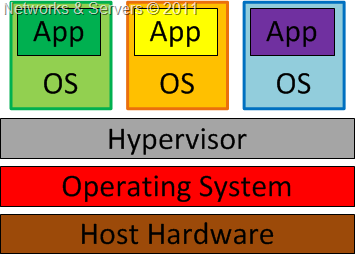
\includegraphics[width=0.5\textwidth]{images/type_2.png}
\end{center}
\end{frame}

\subsection{Embedded Hypervisor}
\begin{frame}
Kernel Level Virtualization - kernel contains extensions designed to manage and control multiple virtual machines. \\
\pause
Examples: KVM
\pause
\begin{center}
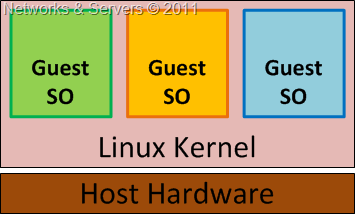
\includegraphics[width=0.5\textwidth]{images/kernel.png}
\end{center}
\end{frame}

\subsection{Advantages}
\begin{frame}
\begin{itemize}
\item truly isolated guest OS
\pause
\item guest OS is not aware of being virtualized
\pause
\item VMM provides standarized hardware environment
\pause
\item full virtualization offers the best isolation and security
\end{itemize}
\end{frame}

\subsection{Disadvantages}
\begin{frame}
\begin{itemize}
\item problem with performance;
\item hypervisor must contain interfaces to resources of machine - device drivers.
\end{itemize}
\end{frame}

\section{Operating System-Level Virtualization}
\subsection{Introduction}
\begin{frame}
Kernel of OS allows for multiple, isolated user-space instances. \\
\pause
Runs on top of existing host. \\
\pause
Provides set of libraries that application interact with. \\
\pause
Provides "illusion" of running on dedicated machine.
\end{frame}

\subsection{Schema}
\begin{frame}
Containers, Virtual Private Servers, Virtual Environments
\pause
Examples: Docker, rkt, OpenVZ, lxc
\pause
\begin{center}
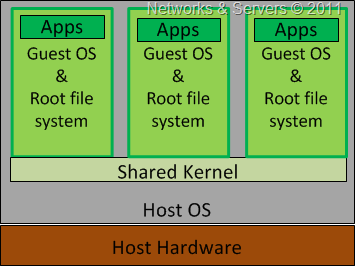
\includegraphics[width=0.5\textwidth]{images/containers.png}
\end{center}
\end{frame}

\subsection{Advantages}
\begin{frame}
\begin{itemize}
\item virtualization usually imposes little to no overhead;
\pause
\item good for webhosting companies with multiple virtual web servers;
\pause
\item patches and modifications are applied once, for every container
\end{itemize}
\end{frame}

\subsection{Disadvantage}
\begin{frame}
\begin{itemize}
\item every guest OS must be identical or similar to host, in terms of version number and patch level
\end{itemize}
\end{frame}

\section{Containers}
\subsection{Origins}
\begin{frame}
\begin{itemize}
\item 14 September 2006: Rohit Seth (Google) provides first version patchset of containers to Linux kernel;
\pause
\item 29 May 2007: Paul Menage, based on Rohit's work, sends updated patchset.
\pause
\item "process containers" changes name to cgroups (control groups) lands in Linux kernel
\pause
\item Linux kernel feature that limits, accounts for, and isolates the resource usage (CPU, memory, disk I/O, network) of a collection of processes.
\end{itemize}
\end{frame}

\subsection{cgroups features}
\begin{frame}
\begin{itemize}
\item provide unified interface
\pause
\item resource limitation: can be set to not exceed configured memory limit;
\pause
\item prioritization: may get larger share of CPU utilization or I/O throughput
\pause
\item accounting: measures how much resources systems use (billing purposes)
\pause
\item control: freezing groups of processes
\end{itemize}
\end{frame}

\subsection{LXC - Linux Containers}
\begin{frame}
LXC combines cgroups and support for isolated namespaces to provide isolated environment for applications. \\
\pause
Originally, LXC containers were not very secure. Before kernel 3.8, root user of guest system, could run code on host system with root privileges. \\
LXC 1.0 (released on 20 February 2014), added "unprivileged containers" - cannot access hardware directly. \\
\pause
LXC 1.0 is intended to be supported for five years. \\
\pause
LXC runs on vanilla Linux kernel.
\end{frame}

\subsection{Docker}
\begin{frame}
Docker was released as open source in March 13, 2013. \\
\pause
Used LXC as default execution environment. \\
\pause
With Docker 0.9 release (March 10, 2014), Docker changes default LXC to libcontainer (written in Go, to access kernel's container APIs directly).
\end{frame}

\subsection{rkt}
\begin{frame}
At September 7, 2013 Docker removed manifest with informations about "standard container" assumptions. \\
CoreOS starts with rkt (rocket) to provide standarized format for containers:
\pause
\begin{itemize}
\item composable: all tools downloadable, but independent and composable
\pause
\item security: isolation should be pluggable
\pause
\item image distribution
\pause
\item open: format and runtime should be well-specified and developed by a community.
\end{itemize}
\pause
rkt 0.1.0 released at December 1, 2014.
\end{frame}

\subsection{Foundations}
\begin{frame}
\textit{Open Container Initiative} \\
On June 22, 2015 at Dockercon there was an information about "Open Container Project". Initiative to gather all companies around containers and protect from fragmentation. \\
--  \\
\textit{Cloud Native Computing Foundation} \\
On July 21, 2015 19 companies created open source foundation. Foundation aims to specify how clouds should be architected to serve modern applications.
\end{frame}

\section{Bibliography}
\begin{frame}
\begingroup
\fontsize{6pt}{8pt}\selectfont
\begin{itemize}
\item Networks \& Servers: \url{http://networksandservers.blogspot.com/2011/11/server-virtualization-explained.html}
\item Origins: \url{http://lwn.net/Articles/236038/}
\item cgroups: \url{https://en.wikipedia.org/wiki/Cgroups}
\item cgroups redesign: \url{http://www.linux.com/news/featured-blogs/200-libby-clark/733595-all-about-the-linux-kernel-cgroups-redesign}
\item LXC: \url{https://en.wikipedia.org/wiki/LXC}
\item Docker: \url{https://en.wikipedia.org/wiki/Docker_(software)}
\item Docker 0.9: \url{https://blog.docker.com/2014/03/docker-0-9-introducing-execution-drivers-and-libcontainer/}
\item rkt: https://coreos.com/blog/rocket/
\item Open Container Initiative: \url{https://www.opencontainers.org/pressrelease/}
\item Innovation or revolution?: \url{https://www.virtualizationpractice.com/containers-innovation-evolution-will-rule-world-34069/?PageSpeed=noscript}
\end{itemize}
\endgroup
\end{frame}

\end{document}
